\documentclass[11pt]{article}

\usepackage{amsmath}
\usepackage{amsfonts}
\usepackage{url}
\usepackage{graphicx}
\usepackage[a4paper,top=1.2in, bottom=1.2in, left=1.2in, right=1.2in]{geometry}
\usepackage{ifthen}
\usepackage{xspace}
\usepackage{tikz}

% no indent
\setlength\parindent{0pt}

% points
\newcommand{\points}[1]{
    \ifthenelse{\equal{#1}{1}}
        {\\ \emph{(#1 Point)}}
    % else
        {\\ \emph{(#1 Points)}}
}

\newcommand{\mat}[1]{
    \mathbf{#1}
}
\newcommand{\argmax}{\operatornamewithlimits{arg\,max}}
\def\IR{\mathbb{R}}
\def\IE{\mathbb{E}}
\def\ie{\emph{i.e.}\@\xspace}

\begin{document}

\begin{center}
\textbf{Exercise for MA-INF 2201 Computer Vision WS19/20\\
15.12.2019\\
Submission until 04.01.2020\\
Christmas Special}\\
\end{center}

\vspace{1cm}

\begin{enumerate}
    % exercise 1
    \item \textbf{Convolution and Fourier Transform:}
    \begin{enumerate}
        % 1 a
        \item Compute the Fourier transform of the function
              \begin{align*}
                  r(t) = \begin{cases} k, |t| \leq a/2, \\ 0, |t| > a/2. \end{cases}
              \end{align*}
        \points{2}
        % 1 b
        \item Below you see a frequency spectrum of an image. The frequency magnitudes are color coded, \ie red is a high value, blue a low value.
              \begin{center}
                  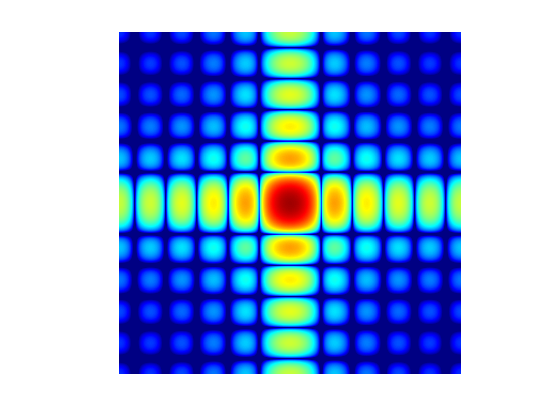
\includegraphics[scale=0.5]{img/fourier1.png}
              \end{center}
              How did the original image look like? Explain why.
        \points{1.5}
        % 1 c
        \item With which function does convolution keep the frequencies of a signal $ s(t) $ (or image $ I(x,y) $) unchanged? Why?
        \points{1}
        % 1 d
        \item For the following $ 5 \times 5 $ filter, determine if it separable. If yes, provide a separation. If not, argue why not.
              \begin{align*}
                  A = \begin{pmatrix}
                         3 & 1 & -9 & -2 & 0 \\
                         5 & 2 & 2 & 3 & -1 \\
                         9 & 4 & -9 & -8 & 1 \\
                         2 & 10 & -20 & -20 & 0 \\
                         4 & 8 & 4 & -6 & 0
                      \end{pmatrix}
              \end{align*}
        \points{1}
        % 1 e
        \item For the following $ 5 \times 5 $ filter, determine if it separable. If yes, provide a separation. If not, argue why not.
              \begin{align*}
	              A = \begin{pmatrix}
	                -21 & 6 & 3 & 12 & 9 \\
	                7 & -2 & -1 & -4 & -3 \\
	                0 & 0 & 0 & 0 & 0 \\
	                35 & -10 & -5 & -20 & -15 \\
	                -14 & 4 & 2 & 8 & 6
                  \end{pmatrix}
          \end{align*}
        \points{1}
        % 1 f
        \item Compute the $ 2 $D distance transform of the below image by hand.\\
              \begin{center}
              
\begin{tikzpicture}[scale=0.5]
                  \fill[black!50] (0,7) rectangle (8,8);
                  \fill[black!50] (3,3) rectangle (5,8);
                  \fill[black!50] (2,2) rectangle (3,4);
                  \fill[black!50] (5,2) rectangle (6,4);
                  \fill[black!50] (1,1) rectangle (2,3);
                  \fill[black!50] (6,1) rectangle (7,3);
                  \fill[black!50] (0,0) rectangle (1,2);
                  \fill[black!50] (7,0) rectangle (8,2);
                  \draw[step=1cm,gray,thick] (0,0) grid (8,8);
              \end{tikzpicture}
              \end{center}
              Provide the result after the initialization, after the forward pass, and after the backward pass.
        \points{2.5}
    \end{enumerate}

    % exercise 2
    \item \textbf{EM-Algorithm and Factor Analysis}:
    When working with images, a normal distribution with a full covariance matrix is usually prohibitive since images are of very high dimension. A $ 100 \times 100 $ pixel image already requires
    a $ 10,000 \times 10,000 $ covariance matrix. Using a diagonal covariance matrix only can be too strong a limitation. \textit{Factor analysis} provides a compromise by adding additional
    degrees of freedom to the model without using the full covariance matrix. Assuming $ D $-dimensional observations, a matrix $ \mathbf{\Phi} \in \IR^{D \times K} (K \ll D) $ is
    used to extend the diagonal covariance matrix $ \mat{\Sigma} \in \IR^{D \times D} $. The final model then looks as follows:
    \begin{align}
        Pr(x) = \mathcal{N}_{x}(\mu, \mat{\Phi}\mat{\Phi}^T + \mat{\Sigma}).
        \label{factorAnalysis}
    \end{align}
    We define
    \begin{align}
        Pr(x|h) &= \mathcal{N}_{x}(\mu + \mat{\Phi}h, \mat{\Sigma}), \\
        Pr(h)   &= \mathcal{N}_{h}(0,\mat{I}).
    \end{align}
    Then, Equation \eqref{factorAnalysis} can be rewritten as a marginalization by introducing a $ K $-dimensional hidden variable $ h $,
    \begin{align}
        Pr(x) &= \int Pr(x|h) Pr(h) dh \nonumber \\
              &= \int \mathcal{N}_{x}(\mu + \mat{\Phi}h, \mat{\Sigma}) \mathcal{N}_{h}(0,\mat{I}) dh.
        \label{marginalization}
    \end{align}
    Note that Equation \eqref{factorAnalysis} and \eqref{marginalization} are equivalent formulations of the same problem. Equation \eqref{marginalization} allows us to optimize the model
    parameters using the EM-Algorithm.
    \begin{enumerate}
        % 2 a
        \item Given observations $ x_1,\dots,x_i,\dots,x_I $, derive the E-Step of the EM-Algorithm for factor analysis, \ie compute
              \begin{align*}
                  \hat q_i(h_i) = Pr(h_i | x_i, \theta),
              \end{align*}
              where $ \theta = (\mu, \mat{\Phi}, \mat{\Sigma}) $ denotes the set of model parameters.
              \textit{Hint:} Terms that are independent of $ h_i $ are irrelevant later in the M-Step, so you can just represent them in a constant.
        \points{2}
        % 2 b
        \item Show that the update rules are
              \begin{align*}
                  \tilde \mu         &= \frac{1}{I} \sum_{i=1}^I \big( x_i - \mat{\tilde \Phi} \IE(h_i) \big), \\
                  \mat{\tilde\Phi}   &= \Big( \sum_{i=1}^I (x_i - \tilde \mu) \IE(h_i)^T \Big) \Big( \sum_{i=1}^I \IE(h_ih_i^T) \Big)^{-1}, \\
                  \mat{\tilde\Sigma} &= \frac{1}{I} \sum_{i=1}^I \mathrm{diag} \Big[ (x_i - \tilde \mu)(x_i - \tilde \mu)^T - \mat{\tilde\Phi} \IE(h_i)(x_i - \tilde \mu)^T \Big].
              \end{align*}
              To make it easier, you may use that:
              \begin{align*}
                   & \argmax_{\tilde \theta} \Big\{ \sum_{i=1}^I \int \hat q_i(h_i) \log Pr(x_i,h_i|\tilde \theta) dh_i \Big\} \\
                  =& \argmax_{\tilde \theta} \Big\{ \sum_{i=1}^I \IE \big[ -\log |\mat{\tilde \Sigma}| - (x_i - \tilde \mu - \mat{\tilde \Phi}h_i)^T \mat{\tilde \Sigma}^{-1}
                                                                                                    (x_i - \tilde \mu - \mat{\tilde \Phi}h_i) \big] \Big\}
              \end{align*}
              and
              \begin{align*}
                  \IE(h_i)      &= (\mat{\Phi}^T \mat{\Sigma}^{-1} \mat{\Phi} + \mat{I})^{-1} \mat{\Phi}^T \mat{\Sigma}^{-1} (x_i - \mu), \\
                  \IE(h_ih_i^T) &= (\mat{\Phi}^T \mat{\Sigma}^{-1} \mat{\Phi} + \mat{I})^{-1} + \IE(h_i) \IE(h_i)^T,
              \end{align*}
              where $ \IE $ is the expectation taken with respect to $ Pr(h_i|x_i,\theta) $.
        \points{6}
        % 2 c
        \item What happens to the update rules if $ \mu $ is initialized with the empirical mean, \ie $ \mu^{(0)} = \frac{1}{I}\sum_{i=1}^I x_i $?
        \points{2}
        % 2 d
        \item In order to start with a good initialization, one might want to initialize the model $ \mathcal{N}_x(\mu, \mat{\Phi}\mat{\Phi}^T + \mat{\Sigma}) $ such that it is a normal distribution
              with diagonal covariance, \ie
              \begin{align*}
                  \mu^{(0)} = \frac{1}{I}\sum_{i=1}^I x_i, \quad \mat{\Phi}^{(0)} = \mat{0}, \quad \mat{\Sigma}^{(0)} = \frac{1}{I}\sum_{i=1}^I \mathrm{diag} \big[ (x_i - \mu)(x_i - \mu)^T \big].
              \end{align*}
              Is this beneficial? Why/why not?
        \points{1}
    \end{enumerate}
\end{enumerate}

\end{document}
